\documentclass[10pt,conference]{IEEEtran}

% ============================================================
% CAIN 2027 Research Track submission
% Template: IEEE Conference Proceedings (required by the CAIN 2027 CFP)
% Page limit: 10 pages + up to 2 pages of references
% Double-anonymous: no author names, third-person self-citation,
%   anonymised artifact links.
% Deadline: Fri 30 Oct 2026 (firm).
% ============================================================

\usepackage{booktabs}
\usepackage{graphicx}
\usepackage{amsmath}
\usepackage{enumitem}
\usepackage{listings}
\usepackage[section]{placeins}
\usepackage[hidelinks]{hyperref}
\graphicspath{{figs/}{./}}

% Every reported figure is generated from results/audit_matrix.csv by
% driftaudit.paper_numbers. Do not edit numbers by hand.
% Generated by driftaudit.paper_numbers -- do not edit.
\newcommand{\CleanList}{\texttt{evidently/jensenshannon}, \texttt{evidently/kl\_div}, \texttt{evidently/psi}, \texttt{evidently/wasserstein}, \texttt{reference-psi/status}, \texttt{scipy/wasserstein\_distance}}
\newcommand{\CorroborateExplicit}{19}
\newcommand{\CorroborateNaN}{16}
\newcommand{\CorroborateQuiet}{9}
\newcommand{\CorroborateRaise}{3}
\newcommand{\CorroborateShift}{23}
\newcommand{\CtrlLargeShiftAlarm}{0}
\newcommand{\CtrlLargeShiftDangerous}{2}
\newcommand{\CtrlNoShiftAlarm}{7}
\newcommand{\CtrlNoShiftDangerous}{0}
\newcommand{\DangMissed}{18}
\newcommand{\DangMissedPct}{19\%}
\newcommand{\DangUndefined}{38}
\newcommand{\DangUndefinedPct}{41\%}
\newcommand{\DangUnderpowered}{37}
\newcommand{\DangUnderpoweredPct}{40\%}
\newcommand{\DegenerateDangerous}{4}
\newcommand{\DegenerateNoisy}{23}
\newcommand{\GapHiPP}{27}
\newcommand{\GapLoPP}{9}
\newcommand{\GapPP}{18}
\newcommand{\GuardCells}{168}
\newcommand{\GuardDang}{36}
\newcommand{\GuardImpls}{12}
\newcommand{\GuardPct}{21\%}
\newcommand{\LoloMaxPP}{24}
\newcommand{\LoloMinPP}{11}
\newcommand{\NanReturners}{24}
\newcommand{\NoGuardCells}{210}
\newcommand{\NoGuardDang}{42}
\newcommand{\NoGuardImpls}{15}
\newcommand{\NoGuardPct}{20\%}
\newcommand{\NumCells}{434}
\newcommand{\NumClean}{6}
\newcommand{\NumDangerous}{93}
\newcommand{\NumDetectors}{31}
\newcommand{\NumDivergenceDetectors}{11}
\newcommand{\NumError}{2}
\newcommand{\NumFailAlarm}{8}
\newcommand{\NumFailMiss}{18}
\newcommand{\NumFailNoisy}{53}
\newcommand{\NumFailSilent}{75}
\newcommand{\NumPValueDetectors}{13}
\newcommand{\NumPass}{264}
\newcommand{\NumProbes}{14}
\newcommand{\NumSafeUndefined}{14}
\newcommand{\PctDangerous}{21\%}
\newcommand{\PctDivergence}{10\%}
\newcommand{\PctPValue}{27\%}
\newcommand{\PctStreaming}{38\%}
\newcommand{\PctTutorial}{21\%}
\newcommand{\RateDegenerate}{13\%}
\newcommand{\RateInf}{58\%}
\newcommand{\RateTinyBoth}{65\%}
\newcommand{\RateTinyCurrent}{55\%}
\newcommand{\SilentZeroCells}{14}
\newcommand{\SilentZeroDang}{6}
\newcommand{\SilentZeroImpls}{1}
\newcommand{\SilentZeroPct}{43\%}
\newcommand{\SmoothingCells}{42}
\newcommand{\SmoothingDang}{9}
\newcommand{\SmoothingImpls}{3}
\newcommand{\SmoothingPct}{21\%}


\hyphenation{multi-ten-ant re-train-ing di-ver-gence}

\lstset{
  basicstyle=\ttfamily\footnotesize,
  columns=flexible,
  keepspaces=true,
  frame=none,
  aboveskip=4pt,
  belowskip=2pt,
  xleftmargin=6pt,
}

\begin{document}

\title{Silent Failure in Drift Monitoring:\\What Detectors Return When They Cannot Measure}

\author{\IEEEauthorblockN{Anonymous Author(s)}
\IEEEauthorblockA{\textit{Affiliation withheld for double-anonymous review}}}

\maketitle

\begin{abstract}
A production drift monitor is consumed by code, not by a person. A retraining gate written as \texttt{if score >= threshold} treats every value the detector returns as a measurement, so its safety depends entirely on what the detector does when the statistic \emph{cannot be computed}: a reference window that has collapsed to a constant, a window too small to bin, an empty or all-\texttt{NaN} window. If the answer is a small number, the gate is disabled and the dashboard stays green.

We probe \NumDetectors{} detectors---five monitoring libraries and reconstructions of published hand-written implementations---against \NumProbes{} adversarial inputs on which a shift test is undefined or degenerate, and classify every result by what a \emph{caller} could determine from it. In \NumDangerous{} of \NumCells{} cells (\PctDangerous) the caller is handed a value that reads as a valid, unalarming measurement when the test was uncomputable or a real shift was present. The danger tracks the \textbf{kind of statistic}, not the vendor: gates built on p-values are dangerous in \PctPValue{} of cells against \PctDivergence{} for divergence-based gates, because a p-value has no value reserved for ``not applicable'' and its safe-looking end is exactly what an absent sample produces. A static sweep of the same \NumDetectors{} implementations then shows that source-level guards do not help: implementations carrying an explicit guard are dangerous in \GuardPct{} of cells, those with no guard at all in \NoGuardPct{}. Guards cover the cases their authors anticipated, whereas here nothing is undefined in the arithmetic sense---the computation succeeds and returns a legitimate number. The remedy is therefore not more guards but a changed return contract, which we demonstrate costs one field and passes all \NumProbes{} probes.
\end{abstract}

\begin{IEEEkeywords}
drift detection, monitoring, MLOps, API design, conformance testing, silent failure
\end{IEEEkeywords}

% ============================================================
\section{Introduction}
\label{sec:intro}

Deployed models decay as the data they serve shifts, and the standard remedy is to monitor a distribution-shift statistic and retrain when it crosses a threshold~\cite{Gama2014,Bayram2022}. The monitoring literature evaluates such detectors on \emph{detection} quality: detection rate, delay, false-alarm rate under a known shift~\cite{Rabanser2019Failing}. That evaluation assumes the detector is always able to answer.

In production it frequently is not. A feature job fails and a window arrives empty. A reference window is computed at the wrong point in time and every value in it collapses to the same number. A low-volume tenant contributes three observations where the statistic assumes hundreds. In each case the shift test is undefined, but the arithmetic rarely says so: quantile binning on a constant reference silently yields one bin; a two-sample test on three points returns a perfectly well-formed p-value near one.

The consequence is specific to how monitors are consumed. A gate is code:

\begin{lstlisting}[language=Python]
score = detector(reference, current)
if score >= THRESHOLD:
    trigger_retraining()
\end{lstlisting}

\noindent This treats every non-raising return as a measurement. If an undefined test returns a small number, the branch is not taken, no alert is raised, and nothing anywhere records that monitoring stopped working. The failure is invisible precisely because the system behaves exactly as it does when everything is fine.

We know this is not hypothetical because it happened. In a production monitoring harness, a reference window computed at the wrong \texttt{as\_of} collapsed to a constant; the implementation detected that quantile binning could not produce breaks and returned \texttt{0.0}; the retraining trigger it fed never fired, for an entire experiment. The guard was correct about the mathematics and catastrophic about the interface.

This paper asks how widespread that interface property is. We deliberately do \emph{not} ask whether detectors compute good statistics. We ask a weaker, more consequential question:

\begin{quote}
\emph{Given only what the detector returned, could a program distinguish a measurement from a non-measurement?}
\end{quote}

\noindent Our contributions:

\begin{enumerate}[leftmargin=*,itemsep=2pt]
  \item A \textbf{failure taxonomy} for distribution-shift tests---degeneracy, support mismatch, sample size, missingness---realised as \NumProbes{} adversarial probes, each carrying the behaviour a correct detector owes the caller (Section~\ref{sec:probes}).
  \item A \textbf{verdict model} that judges an implementation by what a caller can determine rather than by statistical quality, separating quiet failures from loud ones (Section~\ref{sec:verdicts}).
  \item A \textbf{behavioural audit} of \NumDetectors{} detectors, finding that danger is governed by the kind of statistic rather than by implementation quality (Section~\ref{sec:behaviour}).
  \item A \textbf{static sweep} of the same implementations, with the negative result that source-level guards do not predict behavioural safety (Section~\ref{sec:corpus}).
  \item A \textbf{constructive fix} and its cost (Section~\ref{sec:fix}).
\end{enumerate}

% ============================================================
\section{Background and Related Work}
\label{sec:related}

\subsection{Drift detection and its evaluation}

Gama et al.\ survey concept drift adaptation~\cite{Gama2014}; Bayram et al.\ review detectors aimed at practical deployment~\cite{Bayram2022}. Rabanser et al.\ evaluate shift-detection methods empirically and, as the title suggests, argue for failing loudly~\cite{Rabanser2019Failing}---our concern is the case where a detector has nothing to be loud about because it believes it succeeded. The Population Stability Index originates in credit scoring~\cite{Lewis1994CreditScoring}; its statistical properties, including instability at small samples, are characterised by Yurdakul and Naranjo~\cite{YurdakulNaranjo2020,Yurdakul2018Thesis}. Streaming detectors such as ADWIN~\cite{Bifet2007ADWIN}, KSWIN~\cite{Raab2020KSWIN} and Page-Hinkley~\cite{Page1954} address the same problem under a different contract, and ship in River~\cite{Montiel2021River}. Klaise et al.\ argue for treating monitoring as a first-class production concern~\cite{Klaise2020Monitoring}, a position the Alibi Detect library implements~\cite{AlibiDetect}. The other implementations we audit are Evidently~\cite{Evidently}, NannyML~\cite{NannyML}, and the general-purpose two-sample tests in SciPy~\cite{Virtanen2020SciPy}, which ships no drift detector but whose tests are routinely wired into gates.

Across this literature, detector quality is measured by how well a detector distinguishes shift from no shift. We measure something orthogonal: whether it distinguishes either from \emph{cannot tell}.

\subsection{Data validation and production ML}

Sculley et al.\ identify monitoring as a locus of hidden technical debt~\cite{Sculley2015}, and Breck et al.\ propose a production-readiness rubric that includes tests for monitoring infrastructure~\cite{Breck2017}. Data-validation systems such as TFX's~\cite{Baylor2017TFX,Polyzotis2019} check inputs against a schema before they reach a model. These are complementary: a validation layer that catches empty or malformed windows would prevent some of our probes from ever reaching a detector. Our results describe what happens when it does not---which is the common case, because drift monitors are typically wired directly to a feature store, and because a half-missing window is schema-valid.

\subsection{Silent failure as a software fault}

The pattern generalises a known class of software fault. Yuan et al.\ show that a large share of catastrophic distributed-system failures stem from trivially incorrect error handling, frequently an empty or over-broad handler~\cite{Yuan2014Simple}, and Ebert et al.\ characterise exception-handling bugs in Java~\cite{Ebert2015Exceptions}. Studies of machine-learning code find related defect classes in TensorFlow and deep-learning programs~\cite{Zhang2018Empirical,Islam2019Repair}. Our contribution to that line is a domain where the fault is not a bad handler but an impoverished \emph{return type}: there is no handler to write, because nothing goes wrong.

The API dimension is the one most directly implicated. Conflating ``absent'' with ``zero'' in a return value is a recognised interface smell---the same defect that motivates option and result types in language design, and that Hoare characterised as the cost of a null reference. Our results give it an empirical footing in one domain: the conflation is not an occasional oversight but the default across \NumDetectors{} implementations from five independent projects, and adding the missing case costs one field.

\subsection{Testing systems without a reference output}

Machine-learning components resist conventional testing because the correct output is often unknown. Two responses are relevant here. Metamorphic testing sidesteps the missing oracle by asserting relations between inputs and outputs rather than absolute values~\cite{Segura2016Metamorphic}, and production-readiness rubrics prescribe process-level checks, including tests of the monitoring infrastructure itself~\cite{Breck2017}. Our battery is a third, narrower instance: we need neither a correct drift score nor a metamorphic relation over scores, only the observation that certain inputs admit \emph{no} correct score, which turns an oracle problem into a conformance-testing problem. Site-reliability practice makes the complementary point from the operations side, where a monitor that has stopped reporting must be distinguishable from a monitor reporting that all is well. Drift monitoring, as our results show, largely lacks that distinction.

% ============================================================
\section{Method}
\label{sec:method}

\subsection{The evaluation target: a gate contract}
\label{sec:contract}

We are not evaluating whether a statistic answers its own question correctly. We evaluate implementations against the contract imposed by the way they are used, which we state explicitly:

\begin{quote}
A \emph{drift gate} maps a reference window and a current window to one of three outcomes: \textsc{drift}, \textsc{no drift}, or \textsc{cannot determine}. The third must be distinguishable from the second by a program with access only to the return value.
\end{quote}

This is a stronger requirement than the statistical literature places on a two-sample test, and deliberately so. A test asked ``is there evidence against the null?'' answers correctly when it returns a large p-value for three observations. A gate asked ``should I retrain?'' must not answer ``no'' on that basis, because ``no evidence of change'' and ``no ability to detect change'' license entirely different operational responses: one is reassurance, the other is an alarm about the monitoring pipeline.

Our results should therefore be read as: \emph{how often does this implementation, used as a gate, violate the gate contract?}---not as a claim that any library is statistically incorrect. Where a library documents that it implements a hypothesis test and nothing more, the violation belongs to the integration, and the fix in Section~\ref{sec:fix} is one the library can supply cheaply on the caller's behalf.

\subsection{Undefined versus underpowered}
\label{sec:undef-vs-underpowered}

Within the probes a gate cannot answer, two distinct situations arise, and we keep them separate because the strength of the claim differs.

\emph{Arithmetically undefined}: the computation has no value. Quantile binning on a constant reference yields fewer than two edges; an empty window has no proportions; every value is \texttt{NaN}. No convention makes a number the right answer. Probes: constant reference, empty current, all-\texttt{NaN} current.

\emph{Well-defined but underpowered}: the arithmetic succeeds and the statistic is valid, but at $n{=}3$ or $n{=}5$ it cannot discriminate, and published thresholds calibrated asymptotically do not govern it~\cite{YurdakulNaranjo2020}. A test returning a large p-value here is right about its own question. Our contract still counts a quiet answer as a violation, because the gate cannot distinguish it from stability---but a reviewer who rejects the contract would rightly discount these cells.

The distinction is material, so we give the split rather than assert it. Of the \NumDangerous{} dangerous cells, \DangUndefined{} (\DangUndefinedPct{}) are arithmetically undefined, \DangUnderpowered{} (\DangUnderpoweredPct{}) are well-defined but underpowered, and \DangMissed{} (\DangMissedPct{}) are genuine shifts reported as stable. No class holds a majority. A reader who rejects the gate contract for underpowered inputs should discount \DangUnderpoweredPct{} of our dangerous cells; the remaining \NumDangerous{} minus \DangUnderpowered{} stand on the narrower reading alone.

\subsection{Gate thresholds}
\label{sec:thresholds}

Every verdict depends on how a score becomes a decision, so the thresholds are fixed in one place (Table~\ref{tab:thresholds}) and are conventional rather than tuned.

\begin{table}[t]
\caption{Decision rules. Library-native thresholds are used where a library computes its own.}
\label{tab:thresholds}
\footnotesize
\begin{tabular}{@{}lll@{}}
\toprule
\textbf{Statistic} & \textbf{Rule} & \textbf{Source} \\
\midrule
p-value tests   & $p < 0.05$          & conventional $\alpha$ \\
PSI             & $\ge 0.15$          & between the 0.1/0.25 \\
                &                     & rule-of-thumb bands \\
Raw distances   & $d/\sigma_{\mathrm{ref}} \ge 0.25$ & dimensionless effect size \\
Evidently       & library default per test & library \\
NannyML         & library-derived alert    & library \\
River           & detector's own boolean   & library \\
\bottomrule
\end{tabular}
\end{table}

Raw distances require care. Wasserstein and energy distance are expressed in the data's own units, so an absolute cut-off is meaningless: the Wasserstein distance between two samples of $\mathcal{N}(100, 15)$ is about $1.9$, which any small fixed threshold would flag as drift. We normalise by the reference standard deviation and gate on a dimensionless effect size. When the reference is degenerate the normaliser is itself undefined, and the adapter reports that rather than dividing by zero---a decision that, we note, is exactly the discipline this paper asks of libraries.

\subsection{Probes}
\label{sec:probes}

A probe is a pair of samples $(\mathrm{reference}, \mathrm{current})$ together with the behaviour a correct detector owes the caller. We group \NumProbes{} probes into four failure classes and two controls (Table~\ref{tab:probes}).

\begin{table}[t]
\caption{The probe battery. \textsc{u}~=~undefined, \textsc{sh}~=~shifted, \textsc{st}~=~stable.}
\label{tab:probes}
\footnotesize
\begin{tabular}{@{}llc@{}}
\toprule
\textbf{Class} & \textbf{Probe} & \textbf{Owed} \\
\midrule
Degeneracy & reference constant, current varies & \textsc{u} \\
           & current constant, reference varies & \textsc{sh} \\
           & both constant, equal & \textsc{st} \\
           & both constant, different & \textsc{sh} \\
\addlinespace
Support    & current outside reference range & \textsc{sh} \\
           & current fills a reference gap & \textsc{sh} \\
\addlinespace
Sample size & current $n{=}3$ & \textsc{u} \\
            & both $n{=}5$ & \textsc{u} \\
            & current empty & \textsc{u} \\
\addlinespace
Missingness & current all \texttt{NaN} & \textsc{u} \\
            & current half \texttt{NaN} & \textsc{u} \\
            & current contains $\infty$ & \textsc{u} \\
\addlinespace
Control    & same distribution & \textsc{st} \\
           & mean shifted $>2\sigma$ & \textsc{sh} \\
\bottomrule
\end{tabular}
\end{table}

The owed behaviour is set from first principles about the data situation, not by majority vote among implementations. Two probes admit reasonable disagreement, and both were identified before any result was inspected; Section~\ref{sec:sensitivity} shows neither affects a conclusion.

Each probe corresponds to a condition a production monitor meets and a benchmark does not:

\begin{description}[style=unboxed,leftmargin=0pt,itemsep=2pt]
  \item[Degeneracy.] A reference window whose values are all identical. This is the signature of a feature computed at the wrong point in time---a window aggregating the last seven days, evaluated at a moment when no observation falls inside it, yields the same zero for every entity. Quantile binning then produces fewer than two distinct edges and any binned divergence is undefined.
  \item[Support mismatch.] The current window occupies a region where the reference has no mass. Bin-wise ratios involve division by zero unless the implementation smooths, and the smoothing constant---not the data---then determines the reported severity.
  \item[Sample size.] A low-traffic segment, a new tenant, or the first hour of a reporting period supplies a handful of observations. Three points cannot populate ten bins, and the published PSI thresholds of $0.1$ and $0.25$ are asymptotic~\cite{YurdakulNaranjo2020}: they do not govern a statistic computed from three points, but nothing in the return value says so.
  \item[Missingness.] A partially failed feature job yields a window that is half \texttt{NaN}; an overflow yields infinities. An implementation that drops non-finite values silently halves the effective sample size, changing what the score means without telling anyone.
\end{description}

The two controls exist to keep the battery honest: a detector that simply refuses everything would score well on the failure classes and must be caught failing the controls instead.

\subsection{Verdicts}
\label{sec:verdicts}

Each detector is called on each probe, capturing its return value, any exception, and any warning. The observation is classified by what the caller could determine, then judged against what the probe owed:

\begin{description}[style=unboxed,leftmargin=0pt,itemsep=1pt]
  \item[\textsc{pass}] correct for this probe.
  \item[\textsc{safe-undefined}] declined to answer where an answer was due---uninformative, never dangerous.
  \item[\textsc{fail-silent}] an undefined test reported as a stable measurement.
  \item[\textsc{fail-noisy}] an undefined test reported as drift.
  \item[\textsc{fail-miss}] a real shift reported as stable.
  \item[\textsc{fail-alarm}] no shift reported as drift.
\end{description}

We call \textsc{fail-silent} and \textsc{fail-miss} \textbf{dangerous}: in both, a gate is left believing it measured something and seeing nothing wrong. \textsc{fail-noisy} is deliberately excluded. Reporting drift on an uncomputable test is still incorrect, and a spurious retrain is not free, but it is \emph{visible}: somebody investigates. Grouping it with silent failure would overstate our thesis and would be unfair to implementations that at least fail loudly.

A detector that raises, returns \texttt{NaN}, or returns an explicit status is recorded as safe on that probe regardless of whether an answer was possible. The asymmetry is deliberate: declining to answer never disables a gate.

Warnings are recorded as a separate field rather than as an outcome. A warning does not change the value the caller received, and Python warnings are trivially suppressed and routinely invisible in production logs.

\subsection{Subjects}

We audit \NumDetectors{} detectors: 12 two-sample tests from SciPy wired as gates, 7 Evidently stat tests declaring numeric support, 4 NannyML univariate methods, 3 River streaming detectors, 1 Alibi Detect batch detector, and 4 hand-written PSI implementations. Library adapters are generated from each library's own registry where one exists, so coverage is not chosen after seeing results. Each adapter calls the library as its documentation specifies, and---critically---does \emph{not} pre-check for empty or degenerate input, since the question is what happens when the caller has not thought to check.

\textbf{SciPy is audited as \emph{SciPy-as-gate}, not as a monitoring product.} SciPy ships general-purpose two-sample tests and makes no drift-detection claim; we include them because wiring one directly to a threshold is the most common monitor in practice, and every SciPy result here is a property of that integration rather than a defect in SciPy. We label these rows accordingly throughout.

\textbf{Streaming detectors are driven under a different protocol, and the comparison is weaker for it.} River's ADWIN, KSWIN and Page-Hinkley consume one observation at a time and expose a boolean drift state; they have no two-window contract. We feed the reference window observation by observation, then the current window, and record whether drift was signalled at any point during the current window. This is a defensible reading of ``did this window drift'', and matches how a batch-oriented operator would wire a streaming detector, but it is our construction rather than the library's documented use. Two consequences follow. Their detectors never see the multi-window history that adaptive windowing is designed to exploit, and an empty or three-point current window gives them almost nothing to update on. We therefore treat the streaming rate (Section~\ref{sec:behaviour}) as \textbf{indicative and protocol-dependent}, exclude streaming detectors from the family-gap comparison that carries our central claim, and flag a dedicated streaming protocol as the clearest extension of this work.

The four hand-written implementations carry different evidential weight and are reported separately throughout. Two reconstruct patterns from published sources: quantile bins with zero cells replaced by a small constant, and fixed-width bins. Both are attested in a widely referenced public PSI repository and in tutorial write-ups. One is the field defect described in Section~\ref{sec:intro}; a search of published implementations did not find that pattern, so it is reported as a single observed instance and never as a rate. The fourth is our reference implementation, a positive control.

\textbf{We do not claim} to have measured how common any pattern is across practitioner code at large; that would require a repository sample we did not collect.

% ============================================================
\section{Behavioural Results}
\label{sec:behaviour}

Across $\NumDetectors \times \NumProbes = \NumCells$ cells, \textbf{\NumDangerous{} (\PctDangerous) are dangerous}: \NumFailSilent{} \textsc{fail-silent} and \NumFailMiss{} \textsc{fail-miss}. A further \NumFailNoisy{} are \textsc{fail-noisy}, \NumFailAlarm{} \textsc{fail-alarm}, \NumSafeUndefined{} \textsc{safe-undefined}, and \NumError{} are errors---both from SciPy on two identical constant windows, where \texttt{epps\_singleton\_2samp} fails to converge and \texttt{anderson\_ksamp} rejects the input for having one distinct observation. Raising is the safe outcome under our contract. The remaining \NumPass{} pass. Figure~\ref{fig:matrix} shows the complete matrix; the block structure by statistic family and the vertical bands at the small-sample and non-finite probes are the two results developed below.

\begin{figure*}[!t]
  \centering
  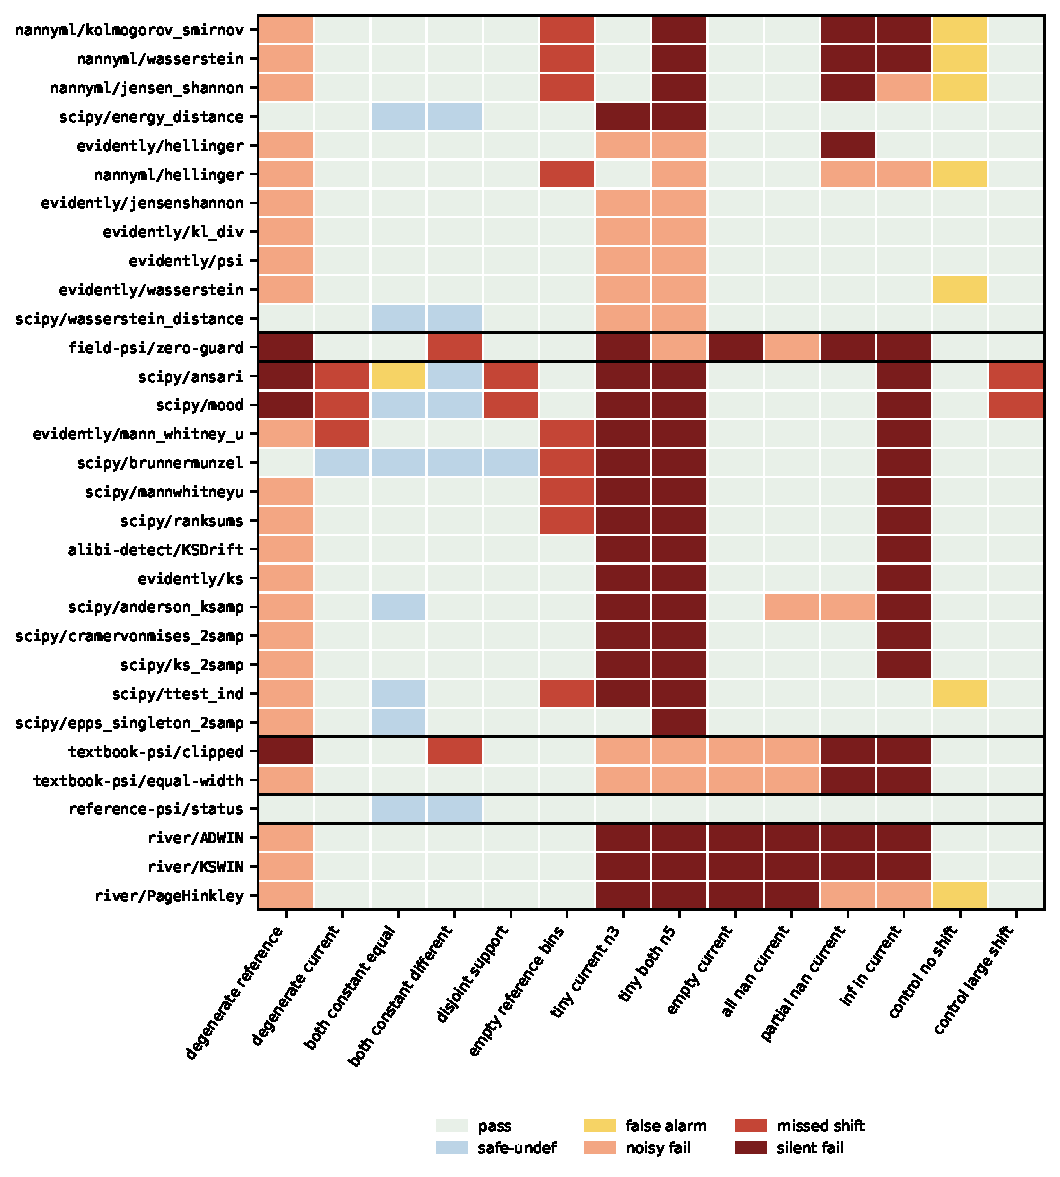
\includegraphics[width=0.78\textwidth]{fig_matrix.pdf}
  \caption{The complete audit matrix. Rows are detectors grouped by statistic family (horizontal rules), columns are probes. Dark cells are dangerous: the caller was handed a value reading as a valid, unalarming measurement when the test was uncomputable or a real shift was present. Danger forms horizontal blocks (families) and vertical bands (small samples, non-finite values); the large-shift control is missed by \CtrlLargeShiftDangerous{} scale-only tests and the no-shift control draws \CtrlNoShiftAlarm{} false alarms (Section~\ref{sec:controls}).}
  \label{fig:matrix}
\end{figure*}

\subsection{What a caller actually sees}

One cell makes the mechanism concrete. Probe \emph{current $n{=}3$} supplies a 500-point reference and a three-point current window drawn from the \emph{same} distribution. A two-sample Kolmogorov--Smirnov gate returns a p-value of roughly $0.6$, and the standard gate

\begin{lstlisting}[language=Python]
if ks_2samp(ref, cur).pvalue < 0.05:
    trigger_retraining()
\end{lstlisting}

\noindent does not fire. Every part of this is correct. Three observations genuinely furnish no evidence against the null of no difference, so a large p-value is the right answer to the question the test was asked. But the question the operator meant to ask was ``has this tenant's distribution moved?'', and the honest answer is ``there is not enough data to say''. Those two answers are encoded identically.

Now suppose the three points had come from a wildly shifted distribution. The p-value would still be large, because three points cannot reject anything. The gate is not merely uninformed; it is \emph{unable to fire at all} at this sample size, and it reports that state using the same value it uses for a healthy, stable population measured over months.

\subsection{Danger follows the statistic, not the vendor}

\begin{table}[t]
\caption{Dangerous cells by kind of statistic. The lower two rows are not audited subjects; see text.}
\label{tab:family}
% Generated by driftaudit.paper_numbers -- do not edit.
\begin{tabular}{@{}lrr@{}}
\toprule
\textbf{Statistic family} & \textbf{Dangerous} & \textbf{Rate} \\
\midrule
Streaming detector$^{\dagger}$ & 16/42 & 38\% \\
p-value test & 50/182 & 27\% \\
Published tutorial PSI & 6/28 & 21\% \\
Divergence / distance & 15/154 & \textbf{10\%} \\
\midrule
Field defect ($n{=}1$) & 6/14 & 43\% \\
Reference impl.\ (control) & 0/14 & 0\% \\
\bottomrule
\end{tabular}


\vspace{2pt}
{\footnotesize $^{\dagger}$Driven under our batch protocol, not the library's documented streaming use; indicative only and excluded from the p-value/divergence comparison.}
\end{table}

Table~\ref{tab:family} is the paper's central result. Gates built on \textbf{p-values} are dangerous markedly more often than gates built on \textbf{divergences}---\PctPValue{} against \PctDivergence{}, a gap of \GapPP{} percentage points---and the reason is structural rather than incidental.

\textbf{How firm is that gap?} Our detector set is neither random nor balanced, so we do not offer a significance test. Bootstrapping over \emph{detectors} rather than cells (\NumPValueDetectors{} p-value, \NumDivergenceDetectors{} divergence; 5000 resamples) gives a 95\% interval of $[\GapLoPP, \GapHiPP]$ percentage points, and excluding each library in turn leaves the gap between $+\LoloMinPP$ and $+\LoloMaxPP$ points---smallest when Evidently is removed, largest when NannyML is. The \emph{sign} is stable under every single-library exclusion and that is the claim we make; the magnitude is not precisely estimated, and readers should treat ``markedly more often'' rather than any specific multiple as the finding.

A p-value is a probability under a null hypothesis of no difference. It has no value reserved for ``not applicable'', and---decisively---its safe-looking end is exactly what a degenerate input produces. Three observations furnish no evidence against any null, so the test returns a large p-value, which the gate reads as stability. The statistic is behaving correctly; it is answering a question the caller did not ask.

A divergence is a magnitude of difference against a chosen threshold. Degenerate inputs tend to push these to extremes: an empty or constant window makes a bin-wise ratio blow up rather than vanish. The failure is still wrong, but it lands on the loud side.

The classification criterion is what the \emph{caller consumes}, not the test's origin. NannyML's Kolmogorov--Smirnov method is counted as a divergence because the library exposes the $D$ statistic against its own learned threshold rather than a p-value.

Streaming detectors show the highest rate (\PctStreaming{}), and their contract does compound the problem---a boolean drift state makes ``no drift detected'' and ``never had enough data to decide'' the same value by construction. We nonetheless treat this number as indicative only, because our batch protocol is not their documented use, and we exclude them from the family comparison below.

Two rows in Table~\ref{tab:family} are not audited subjects and their rates are not prevalence estimates (shaded in Fig.~\ref{fig:family}). The field defect is one implementation on \NumProbes{} probes---an existence proof. The reference implementation is our own control, discussed in Section~\ref{sec:fix}.

\begin{figure}[!t]
  \centering
  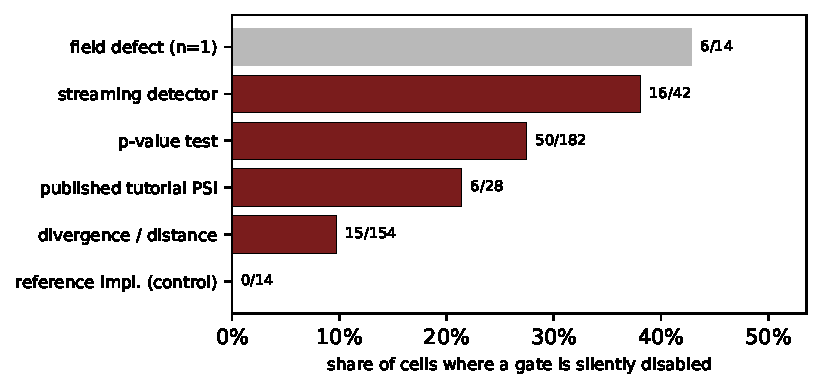
\includegraphics[width=\columnwidth]{fig_family.pdf}
  \caption{Dangerous cells by statistic family. Hatched bars are not audited subjects: one observed field defect and our own positive control.}
  \label{fig:family}
\end{figure}

\subsection{Per-detector results}

\begin{table}[t]
\caption{Dangerous cells per detector, out of \NumProbes{} probes each. Detectors with no dangerous cell are listed first.}
\label{tab:detectors}
\footnotesize
% Generated by driftaudit.paper_numbers -- do not edit.
\begin{tabular}{@{}lr@{\hspace{1.2em}}lr@{}}
\toprule
\textbf{Detector} & \textbf{D} & \textbf{Detector} & \textbf{D} \\
\midrule
\texttt{evidently/jensenshannon} & 0 & \texttt{scipy/ks\_2samp} & 3 \\
\texttt{evidently/kl\_div} & 0 & \texttt{scipy/ttest\_ind} & 3 \\
\texttt{evidently/psi} & 0 & \texttt{nannyml/kolmogorov\_smirnov} & 4 \\
\texttt{evidently/wasserstein} & 0 & \texttt{nannyml/wasserstein} & 4 \\
\texttt{reference-psi/status} & 0 & \texttt{river/PageHinkley} & 4 \\
\texttt{scipy/wasserstein\_distance} & 0 & \texttt{scipy/brunnermunzel} & 4 \\
\texttt{evidently/hellinger} & 1 & \texttt{scipy/mannwhitneyu} & 4 \\
\texttt{nannyml/hellinger} & 1 & \texttt{scipy/ranksums} & 4 \\
\texttt{scipy/epps\_singleton\_2samp} & 1 & \texttt{textbook-psi/clipped} & 4 \\
\texttt{scipy/energy\_distance} & 2 & \texttt{evidently/mann\_whitney\_u} & 5 \\
\texttt{textbook-psi/equal-width} & 2 & \texttt{field-psi/zero-guard} & 6 \\
\texttt{alibi-detect/KSDrift} & 3 & \texttt{river/ADWIN} & 6 \\
\texttt{evidently/ks} & 3 & \texttt{river/KSWIN} & 6 \\
\texttt{nannyml/jensen\_shannon} & 3 & \texttt{scipy/ansari} & 7 \\
\texttt{scipy/anderson\_ksamp} & 3 & \texttt{scipy/mood} & 7 \\
\texttt{scipy/cramervonmises\_2samp} & 3 &  &  \\
\bottomrule
\end{tabular}

\end{table}

Table~\ref{tab:detectors} gives the per-detector breakdown, and the ordering is itself the finding: the clean end is populated entirely by divergences, the dangerous end almost entirely by p-value tests and streaming detectors. The two worst SciPy-as-gate entries (\texttt{mood}, \texttt{ansari}) test for differences in \emph{scale} rather than location, so the location shift in our control is invisible to them by design---a reminder that ``dangerous'' here is always relative to the drift-gate use, never a claim about a test's own validity (Section~\ref{sec:controls}).

Vendor is a poor predictor. Evidently supplies four of the six cleanest detectors \emph{and} one of the more dangerous (\texttt{mann\_whitney\_u}, 5); SciPy-as-gate supplies one clean entry and the two worst. Within Evidently the split is exactly along our family boundary: its four divergences are clean, its two p-value tests are not. The pattern repeats inside NannyML, whose Hellinger method has one dangerous cell against four for its Kolmogorov--Smirnov and Wasserstein methods.

\subsection{Danger concentrates where production breaks}

\begin{table}[t]
\caption{Every probe, \NumDetectors{} detectors each. \textsc{d}~=~dangerous (silent failure or missed shift); \textsc{n}~=~noisy failure; \textsc{a}~=~false alarm.}
\label{tab:probes-danger}
% Generated by driftaudit.paper_numbers -- do not edit.
\begin{tabular}{@{}lrrrr@{}}
\toprule
\textbf{Probe} & \textbf{\textsc{d}} & \textbf{Rate} & \textbf{\textsc{n}} & \textbf{\textsc{a}} \\
\midrule
Both windows $n{=}5$ & 20 & 65\% & 10 & 0 \\
Current contains $\infty$ & 18 & 58\% & 3 & 0 \\
Current $n{=}3$ & 17 & 55\% & 8 & 0 \\
Current fills reference gap & 9 & 29\% & 0 & 0 \\
Current half \texttt{NaN} & 9 & 29\% & 3 & 0 \\
Reference constant & 4 & 13\% & 23 & 0 \\
Current empty & 4 & 13\% & 2 & 0 \\
Current constant & 3 & 10\% & 0 & 0 \\
Current all \texttt{NaN} & 3 & 10\% & 4 & 0 \\
Both constant, different & 2 & 6\% & 0 & 0 \\
Current outside ref.\ range & 2 & 6\% & 0 & 0 \\
\textbf{Control: large shift} & \textbf{2} & 6\% & 0 & 0 \\
Both constant, equal & 0 & 0\% & 0 & 1 \\
\textbf{Control: no shift} & \textbf{0} & 0\% & 0 & \textbf{7} \\
\bottomrule
\end{tabular}

\end{table}

The distribution across probes (Table~\ref{tab:probes-danger}) is not what the motivating anecdote would predict. \textbf{Degeneracy is comparatively well handled}: a constant reference is dangerous in only \RateDegenerate{} of cells (\DegenerateDangerous{} of \NumDetectors{}) and noisy in \DegenerateNoisy{} more, because most implementations blow up loudly on it. The danger concentrates in \textbf{small samples} (\RateTinyCurrent{}--\RateTinyBoth{}) and \textbf{non-finite values} (\RateInf{} for infinities): exactly the conditions a production monitor meets routinely and a benchmark never does---a low-traffic segment, a partially failed feature job, a window at the start of a reporting period.

\subsection{The controls are not clean, and that is informative}
\label{sec:controls}

\CtrlLargeShiftDangerous{} detectors fail the large-shift control, and \CtrlNoShiftAlarm{} raise a false alarm on the no-shift control. Neither result should be swept into the framing that the battery merely validates itself.

\textbf{\texttt{scipy/mood} and \texttt{scipy/ansari} miss the large shift} ($p = 0.86$ and $0.72$). Both test for a difference in \emph{scale}, and our control shifts the mean while leaving the spread unchanged, so they are blind to it by construction. As statistics they are behaving perfectly; as drift gates they are silently answering a question the operator did not ask. This is the same failure our probes were designed to expose, arriving from an unexpected direction---a reminder that ``dangerous'' throughout this paper is relative to the drift-gate use, never a claim about a test's own validity. It also means the battery is not self-fulfilling: it catches a mismatch we did not plant.

\textbf{\CtrlNoShiftAlarm{} detectors alarm on two samples from the same distribution.} One is \texttt{scipy/ttest\_ind} at $p = 0.038$, which is simply the 5\% false-positive rate a threshold of $\alpha = 0.05$ buys. The other six are the four NannyML methods, \texttt{evidently/wasserstein} and \texttt{river/PageHinkley}, all of which derive or apply thresholds that our single-window protocol stresses (Section~\ref{sec:threats}). These are \textsc{fail-alarm}, excluded from our danger measure by design, and we flag them rather than bury them: a detector that cries wolf on stable data is a real operational problem, just not the one this paper measures.

Six detectors have no dangerous cell: four Evidently tests (\texttt{psi}, \texttt{jensenshannon}, \texttt{kl\_div}, \texttt{wasserstein}), \texttt{scipy/wasserstein\_distance}, and our reference implementation. \textbf{Every one of the five that is not our control is a divergence.}

\subsection{Sensitivity to contested probe expectations}
\label{sec:sensitivity}

Two probes carry judgement calls. Re-deriving the headline under all four labellings:

\begin{table}[t]
\caption{Sensitivity to the two contested expectations.}
\label{tab:sensitivity}
\footnotesize
% Generated by driftaudit.paper_numbers -- do not edit.
\begin{tabular}{@{}llrrr@{}}
\toprule
\textbf{Both const.\ diff.} & \textbf{Half \texttt{NaN}} & \textbf{Overall} & \textbf{p-value} & \textbf{Divergence} \\
\midrule
shifted & undefined & 21\% & 27\% & 10\% \\
shifted & stable & 19\% & 27\% & 7\% \\
undefined & undefined & 21\% & 27\% & 10\% \\
undefined & stable & 19\% & 27\% & 7\% \\
\bottomrule
\end{tabular}

\end{table}

The first choice has \emph{no effect at all}: under \textsc{shifted} a quiet answer is a missed shift, under \textsc{undefined} the same answer is a silent non-measurement, and both are dangerous, so only the name of the failure changes. The second moves the overall rate by two points and \emph{widens} the family gap from 17 to 20 points---the central claim is weakest under the labelling we adopted.

Implementation behaviour independently corroborates both: \CorroborateShift{} of \NumDetectors{} detectors treat two differing point masses as a shift, and \CorroborateExplicit{} of \NumDetectors{} are explicit about a half-missing window (\CorroborateNaN{} return \texttt{NaN}, \CorroborateRaise{} raise) against \CorroborateQuiet{} that quietly report stability.

% ============================================================
\section{Do Source-Level Guards Help?}
\label{sec:corpus}

The behavioural audit measures what implementations do. We now ask how they are written, to test the natural hypothesis that dangerous behaviour reflects missing defensive code.

We resolve each of the \NumDetectors{} audited detectors to the function that actually computes its statistic---from the live callable, not by name matching---and classify the guards in its body by AST analysis: a conditional \texttt{return 0}, a \texttt{NaN} or \texttt{None} return, a \texttt{raise}, clipping or smoothing, or nothing.

\begin{table}[t]
\caption{Static guard classification, and the behavioural danger of the implementations in each class.}
\label{tab:corpus}
% Generated by driftaudit.paper_numbers -- do not edit.
\begin{tabular}{@{}lrr@{}}
\toprule
\textbf{Static class} & \textbf{Impls.} & \textbf{Behavioural danger} \\
\midrule
silent-zero & 1 & 6/14 (43\%) \\
smoothing & 3 & 9/42 (21\%) \\
explicit & 12 & 36/168 (21\%) \\
no-guard & 15 & 42/210 (20\%) \\
\bottomrule
\end{tabular}

\end{table}

Two findings follow (Table~\ref{tab:corpus}).

First, \textbf{the literal return-zero pattern is rare in shipped libraries}---\SilentZeroImpls{} implementation of \NumDetectors{}, and that one is the field defect, not library code. The pattern that motivated this work is a practitioner pattern, not a vendor one.

Second, and more consequentially: \textbf{guards do not predict safety}. Implementations carrying an explicit guard are dangerous in \GuardPct{} of their cells; implementations with no guard whatsoever, in \NoGuardPct{}. The difference is nil.

The explanation is the same structural point as Section~\ref{sec:behaviour}. A guard covers the cases its author anticipated---division by zero, an empty array, a malformed shape. But the silent failure here is not an arithmetic error. Nothing is undefined in the machine sense; no exception is available to catch. The computation \emph{succeeds} and returns a legitimate number that means ``no evidence of difference'' for a sample that carries no evidence of anything. There is nothing for a guard to guard against.

This is why more defensive code is the wrong prescription. Libraries already write it: \GuardImpls{} of \NumDetectors{} implementations we examined carry an explicit signal somewhere in the function, and it buys them nothing measurable.

% ============================================================
\section{The Fix and Its Cost}
\label{sec:fix}

If the problem is that one return channel carries two distinct messages, the fix is to separate them. We implement a reference PSI with arithmetic identical to the common clipped variant, plus one field:

\begin{lstlisting}[language=Python]
@dataclass
class Result:
    score: float | None = None
    flagged: bool | None = None
    status: str | None = None   # the added field
\end{lstlisting}

\noindent \texttt{status} is \texttt{None} when the score is a measurement, and otherwise names why it is not: \texttt{degenerate-reference}, \texttt{insufficient-samples}, \texttt{non-finite-input-dropped-$k$}, \texttt{empty-after-dropping-non-finite}. A gate becomes:

\begin{lstlisting}[language=Python]
r = detector(reference, current)
if r.status is not None:
    escalate_monitoring_gap(r.status)   # not silence
elif r.score >= THRESHOLD:
    trigger_retraining()
\end{lstlisting}

This implementation has \textbf{0 dangerous cells of \NumProbes{}} (Table~\ref{tab:family}), passing 12 probes and declining to answer on 2 where an answer was arguably possible---the conservative direction.

\textbf{We claim this as an existence proof, not a solution.} It shows the failure mode is eliminable at negligible cost, in one implementation of one statistic, evaluated on the same battery it was written against. It is not a solved API-design problem: we have not measured adoption cost in real codebases, migration burden for existing callers, whether operators act on a status they receive, or how the design fares against alternatives such as returning an option type, raising by default with an opt-out, or carrying the diagnostic in a side channel. The status vocabulary itself is ours and unvalidated; a real design would need agreement on the categories. What the control does establish is that the \PctDangerous{} figure is not a floor imposed by the mathematics.

Three design points generalise beyond our implementation:

\begin{enumerate}[leftmargin=*,itemsep=2pt]
  \item \textbf{An undefined score must not be representable as a stable one.} Returning \texttt{NaN} achieves this cheaply, is already done by \NanReturners{} of our \NumDetectors{} detectors on at least one probe, and requires no API change---callers must merely be told to test for it.
  \item \textbf{Sample-size adequacy is part of the result, not the caller's problem.} Published PSI thresholds are asymptotic~\cite{YurdakulNaranjo2020}; a detector that knows $n{=}3$ should say so rather than return a number those thresholds do not govern.
  \item \textbf{Silently dropping non-finite values changes the effective sample size} and therefore the meaning of the score. Reporting how many were dropped costs one integer.
\end{enumerate}

\noindent None of this requires better statistics. It requires that ``I measured stability'' and ``I could not measure'' be different values.

% ============================================================
\section{Implications}
\label{sec:implications}

\subsection{For library authors}

The cheapest correct change is to make the undefined case unrepresentable as a stable one. \NanReturners{} of our \NumDetectors{} detectors already return \texttt{NaN} on at least one probe, so the machinery usually exists; what is missing is that it is not documented as part of the contract, and callers are not told to test for it. A richer status enumerates \emph{why}, which matters because the remedies differ: a degenerate reference is a pipeline bug, an insufficient sample is a scheduling decision, and a half-missing window is an upstream outage.

A second recommendation follows from Table~\ref{tab:probes-danger}. Libraries defend against the failure that is easy to imagine---a constant reference, which blows up visibly---and not against the ones that actually dominate, namely small samples and non-finite values. A minimum-sample parameter with a documented default would convert the single most dangerous column in our matrix into an explicit signal.

\subsection{For practitioners}

The choice of statistic is a choice about failure mode, and it can be made before any tuning. A gate built on a p-value inherits an alarming property: the value that means ``all is well'' is the same value that means ``this test could not run''. If a p-value test is required for other reasons, the gate should be written defensively against the statistic rather than trusting it:

\begin{lstlisting}[language=Python]
if len(cur) < MIN_N or not np.isfinite(cur).all():
    escalate_monitoring_gap()
elif ks_2samp(ref, cur).pvalue < ALPHA:
    trigger_retraining()
\end{lstlisting}

\noindent The precondition check is three lines and is the caller's responsibility today whether or not they know it.

More broadly, a monitor that never alerts is indistinguishable from a monitor that is broken, and our results show that this is not a hypothetical confusion but the default behaviour of a fifth of the configurations we probed. A drift-monitoring deployment should therefore assert liveness independently of drift: record how many windows were scored, how many were skipped, and how many observations each score rested on. None of these are drift statistics; all of them would have caught the field defect that motivated this work.

\subsection{For researchers}

Detector evaluations report detection rate, delay and false-alarm rate under a known shift. We suggest a fourth axis: behaviour when no answer is possible. It is cheap to measure---our battery is \NumProbes{} inputs---and it is not implied by the other three, since a detector can be excellent at discriminating shift from no shift while being unable to express that it did neither.

% ============================================================
\section{Threats to Validity}
\label{sec:threats}

\textbf{Construct.} Our probes are synthetic inputs, not sampled production incidents; we argue they are representative of production conditions but do not demonstrate their frequency. The owed behaviour per probe encodes our judgement about the data situation, mitigated by the sensitivity analysis of Section~\ref{sec:sensitivity} and by the corroboration from implementation behaviour. For one probe---two differing constant windows---the correct expectation is arguably detector-dependent, since Wasserstein distance is well defined on two point masses while PSI has no bins; we retain a single expectation because the sensitivity analysis shows it cannot change a conclusion.

\textbf{Internal.} The dominant error mode of a conformance audit is the auditor, and we report ours in full because a reader cannot otherwise calibrate the rest. Five times we recorded an apparent library defect that was our own mistake: passing a string where an enum was expected; reading the reference row of a two-period result frame, which made a detector appear never to see drift; configuring a library with a single reference chunk, leaving it no variability from which to derive thresholds so that it alarmed on everything; an instrument bug that replaced a detector's verdict with ``warned'' whenever any warning was emitted, discarding the detector's actual answer and inflating one library from 1--4 to 9 dangerous cells; and calling \texttt{anderson\_ksamp(a, b)} when its second positional parameter is a flag rather than a second sample, which invalidated all \NumProbes{} of that detector's cells and was caught only during review. A sixth class---an arbitrary absolute threshold applied to distances expressed in data units---produced spurious false alarms until thresholds were made dimensionless (Section~\ref{sec:thresholds}).

Each was caught by disbelieving a result that looked too bad, which is not a reliable detector of errors that flatter the hypothesis. Readers should weight our numbers accordingly, and anyone replicating this method should budget for it. Mitigations now in place: adapter call surfaces are taken from each library's own signature or registry, per-detector call conventions are declared rather than assumed, every number in Table~\ref{tab:detectors} is machine-checked against the results file by a script in the artifact, and versions are pinned.

\textbf{External.} \NumDetectors{} detectors from five libraries, all Python, all univariate numeric. Multivariate and categorical detectors, and non-Python ecosystems, are unmeasured. The tutorial-PSI row rests on two reconstructions of a documented pattern, not a repository sample, and no prevalence claim is made from it. Two libraries could not be audited under Python 3.13 and required a 3.12 environment; one further library was excluded for an unrelated dependency conflict.

\textbf{Conclusion.} The family effect is descriptive over an unbalanced set---182 p-value cells against 154 divergence cells, drawn from libraries that did not choose their statistics independently. We claim a structural explanation for the gap, supported by the mechanism, not a statistical test over a random sample of detectors.

% ============================================================
\section{Conclusion}
\label{sec:conclusion}

Drift monitors are evaluated on whether they can tell drift from no drift. We asked whether they can tell either from \emph{cannot tell}, and in a fifth of the cases we probed the answer is no: the caller receives a number that reads as a valid, calm measurement when the test was uncomputable or a real shift was present.

Which detector you choose matters less than which \emph{kind of statistic} you build the gate on. A p-value's reassuring end is exactly what an absent sample produces, and gates built on p-values were dangerous markedly more often than gates built on divergences---\PctPValue{} against \PctDivergence{}, with the sign of the gap stable under every single-library exclusion. Nor is the remedy more defensive code: implementations with explicit guards were no safer than implementations with none, because nothing goes wrong for a guard to catch---the arithmetic succeeds and answers a question nobody asked.

What is needed is a return contract in which ``measured, stable'' and ``could not measure'' are different values. That costs one field. For a monitoring component whose entire purpose is to notice when something has changed, being unable to report that it has stopped working is a strange thing to ship, and a cheap one to fix.

% ============================================================
\FloatBarrier
\section*{Data Availability}

An anonymised replication package containing the probe battery, all \NumDetectors{} adapters, the audit and sweep tooling, raw results and pinned environments is available at \url{https://anonymous.4open.science/r/Silent-Failure-in-Drift-Monitoring-4F6D}
during review. Reproducing every table requires only Python and the pinned library versions.

% ============================================================
\section*{Disclosure of Generative AI Use}

In accordance with the ACM Policy on Authorship and the use of generative AI, the authors disclose that a large language model (Anthropic Claude) was used substantially in this work: in drafting and revising the manuscript, in implementing the probe battery, adapters and analysis tooling, and in auditing that tooling for the measurement errors reported in Section~\ref{sec:threats}. All results were produced by executing that code on the authors' infrastructure; no quantitative claim originates from model output. The authors reviewed and take full responsibility for every claim, number, and line of code in the paper and the accompanying artifact.

% ============================================================
\bibliographystyle{IEEEtran}
\bibliography{references}

\end{document}
